\chapter{Unit 2: Energy and Momentum}
\section{Work and Kinetic Energy}
\subsection{Kinetic Energy}
\begin{cyanblock}
    \begin{definition}
        Kinetic energy is the energy of \red{motion}. There are two types of kinetic energy
    \end{definition}
\end{cyanblock}

\subsubsection*{Type 1: Traslational Kinetic Energy}
The kinetic energy that an object has because it is \textit{moving from on location to another}. In can be describe by this 
formula:
\begin{equation}
    E_k = \frac{1}{2}mv^2
\end{equation}
\begin{center}
    $E_k$ is the translational kinetic energy of the object (in $J$ or $kgm^2/s^2$)\\
    $m$ is the mass in $kg$\\
    $v$ is the speed in $m/s$
\end{center}

Because all motion is relative, an object's speed (and therefore $E_k$) \textit{depends on the choose Frame of Reference}\\

\red{Notes:}\\

\red{Do not solve the conservation of energy problem involving a change of Frame of Reference. Start from your perspective}\\

\red{$E_k$ is a scalar, not a vector}

\subsubsection*{Type 2: Rotational Kinetic Energy}
    Not testable, don't give a shit about this qusetion. 

\subsection{Mechancial Work}
\begin{definition}
    Mechanical work: Transfer of energy into $E_k$ or the transfer of kinetic energy into another type of energy
\end{definition}

\begin{definition}
    Potential energy: Energy which is stored in a system of objects due to forces acting in between thos objects
\end{definition}
The formula to descirbe the work is:
\begin{equation}
    W = F_{A/B} * \vec{\Delta d_B} * cos\theta
\end{equation}
\begin{center}
    $W_{A/B}$ is the work that $F_{A/B}$ does on the object $B$. This is also the amount of $E_k$ that object A transfers into object B 
    when A exerts a force on B(in J)\\

    $F_{A/B}$ is the magnitude of force that A exerts on B(in J)\\

    $\theta$ is the angle between $F_{A/B}$ and $B$'s displacement
\end{center}

\red{Remainder: Only forces on the direction of displacement is responsible for the work}

\section{Gravational Potential Energy}
\subsection{Some boring definitions}
\begin{definition}
    (Gravational Potential Energy): The energy storedf in a system of objects due to the force of gravity acting between those objects. In other words, the energy is stored collectively \textbf{among all } the objects in the system
\end{definition}

Whne the force of gravity acting on the two objects causes this stored GPE to be converted into kinetic energy, the kinetic energy is not \textbf{shared evenlly} between these two objects. 
In the class Example, the earth effectively gets \textbf{zero} and the care effectively gets \textbf{all of them}. Due to this reason, when we have two objects with a very large difference in mass, we can 
always assume that the GPE is \textbf{stored only in the smaller object}

\subsection{Formulas for GPE}
\subsubsection*{Formula 1}
\begin{equation}
    \Delta E_g = mg\Delta h
\end{equation}

\begin{center}
    $\Delta E_g$ is the change in Potential gravational energy(in J)\\
    $m$ is the mass of the object (in kg)\\
    $\Delta h$ is the change in height (in m)\\
    $g$ is the acceleration due to gravity (in $m/s^2$)
\end{center}

\subsubsection*{Fromula 2}
\begin{equation}
    E_g = mg\Delta h
\end{equation}
\begin{center}
    $E-g$ is related to the GPE of the object
\end{center}

\begin{remark}
    For all questions related to the \textbf{Gravational Potential Energy}, you must set your reference height in the diagram. Or, Mr McCumber will forget to add 0.5 for your test!
\end{remark}

\section{The law of the Conservation of Energy}
\subsection{Boring Definitions}
\begin{definition}
    (Law of the Conservation of Energy): Energy will neither created or destroy, only change from one form to another
\end{definition}

\begin{remark}
    The law of the conservation of energy only works in a \textbf{closed isiolated} system. In reality, the only true \textbf{closed and isolated} system is the Universe
\end{remark}

\subsubsection*{Mechancial Energy}
\begin{definition}
    (Mechancial Energy): is the sum of the \textbf{kinetic energy} and g\textbf{gravational potential energy}.
\end{definition}

Mathematically:
\begin{equation}
    E_m = E_g + E_k
\end{equation}

\subsection{Question solving techniques}
When you solve a question about conversation of energy, always write this:
\begin{gather}
    E_{m1} = E_{m2}\\
    E_{k2} + E_{g2} = E_{k1} + E_{g1} + W_{ap} + W_{f}
\end{gather}

Then, cross out terms which equal to \textbf{zero}

\begin{remark}
    Remember to write this, or teacher will forget to add your marks!
\end{remark}

\section{String \& Elastic Potential Energy}
\subsection{The Force of String}
\begin{definition}
    (Spring Force): Can be wrote as $F_{spring}$. It is the force exerted by the spring on a object. 
\end{definition}

According to the Hooke's Law, the \textbf{force exerted by a string} is proportional to the string's displacement. So we can express the relationships between
them by some formulas:\\

Vector Version:
\begin{gather}
    \vec{F_x} = -k\Delta \vec{x}
\end{gather}

Scalar Version:
\begin{gather}
    F_x = k \Delta x
\end{gather}

\begin{center}
    $F_x$ is the force exerted by the string on whatever stretches it.\\
    $k$ is the constant of string\\
    $x$ is the displacement of the spring from its unstratched
\end{center}

An essential feature of Hooke's law is that the direction of the spring force is \textbf{opposite} to the direction of displacement from equilibrium. 

\begin{remark}
    When you use the Scalar version, you must clearly understand the direction of the force in you heart. 
\end{remark}

\newpage
\subsubsection*{Deeper explanation about Hooke's law}
\begin{figure}[h!]
    \centering
    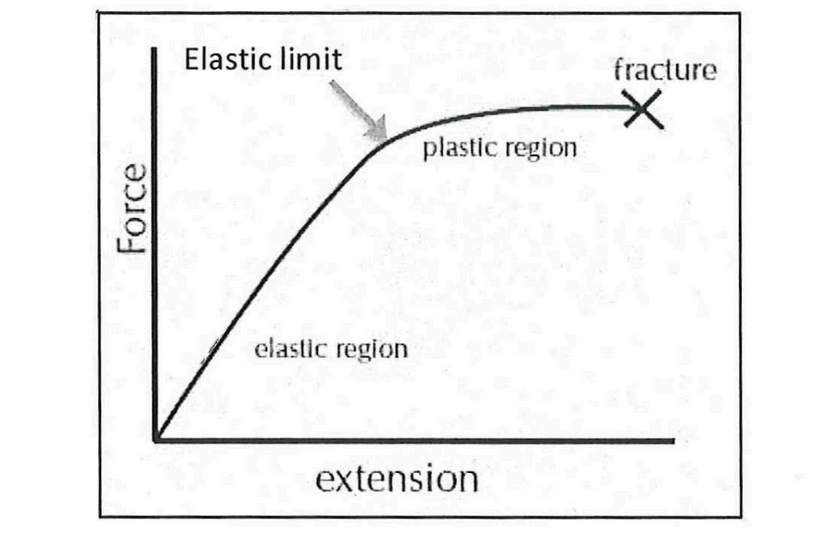
\includegraphics[width=0.5\textwidth]{graph/Hooke's Law.png}
\end{figure}

\begin{definition}
    (Elastic Region): Elastic objects obey Hooke's Law in this region. If the applied force removed, the object will naturally 
    return back to its original shape
\end{definition}

\begin{definition}
    (Elastic Limit): The maximum amount of deformation an object can withstand, and still return to its original shape. 
\end{definition}

\begin{definition}
    (Plastic region): The object no longer obeys Hooke's Law. The object's shape is now permanetly changed. 
\end{definition}

\begin{definition}
    (Fracture): The maximum amount of shape change the object can take, prior to failing (breaking).
\end{definition}

\subsection{Elastic Potential Energy}
\begin{definition}
    (elastic potential energy): The potential energy due to the stretching or compressing of an elastic material
\end{definition}

\begin{figure} [h!]
    \centering
    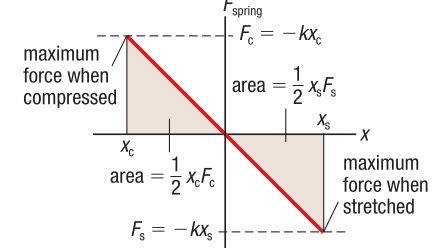
\includegraphics[width=0.5\textwidth]{graph/elastic Potential energy.png}
    \caption{The work done by a variable force is equal to the area under the the force-displacement graph}
\end{figure}

\subsubsection*{Formula}
\begin{gather}
    W = \frac{1}{2} * \Delta x * F_{spring}\\
    W = \frac{1}{2} * \Delta x * (k * \Delta x)\\
    W = \frac{1}{2} * k * (\Delta x)^2
\end{gather}

The work done by the spring force is the negative of this amount, and is also the negative of the change in Potential Energy.
That means that the work done stretching or compressing the spring is transformed into elastic potential energy.
\begin{equation}
    E_e = \frac{1}{2} k (\Delta x)^2
\end{equation}